\documentclass[10pt,a4paper,titlepage]{article}
%\documentclass[10pt,a4paper,titlepage]{book}
%\documentclass[11pt,a4paper,titlepage]{report}


\usepackage{inc/ltfs}
%\usepackage{generatedoc}
\usepackage{xkeyval}
\usepackage{calc}%一个可以在tikz中直接计算位置的包
\usepackage{xxcolor}
\usepackage{pifont}
\usepackage{makeidx}


\begin{document}
\pagestyle{plain}%plain页面格式
\pagenumbering{roman}%罗马字母计数

\title{\Huge{例学Tikz\& PGF}\\ \vspace{10pt}---\large{pgf manual封面设计源码分析}}
\date{\modeldate}
\author{
\Huge{%\Kunstler
\modelauthornet}
\includegraphics[width=1.68em]{pic/byrlogo.png}
}
\maketitle

\tableofcontents


\listoffigures

\clearpage
\phantomsection
\addcontentsline{toc}{section}{Abstract}

\begin{abstract}

本篇文档从PGFmanual.pdf的封面设计源码出发,介绍了一些关于pgf和tikz绘图的实例。阅
读本篇文档并不要求你精通pgf\footnote{实际上如果你精通的话也不用来看这个了},你只
需要把lnotes上关于pgf绘图部分弄懂,就可以无障碍\footnote{还要懂英文哦}地读完整
篇文档了。

文档将pgfmanual封面的代码划分为几个部分,依次贴出了代码以及对代码的解读,其中也
夹杂着我对tikz绘图的一些看法和总结。这几个部分包含了pgf作图常用到的坐标系建立,
定位,渐变色绘制等常用的方法,并且包含了倒影文字,雪花以及脚印修饰三种艺术性的装
饰方法。很多的属性或者方法,本文档都给出了其在pgfmanual中具体介绍的页面位置,你
可以直接翻到指定的地方去研究更多的东西。需要注明的是本文所指的pgfmanual全部均为
/texmf-dist/doc/generic/pgf/pgfmanual.pdf文件,而且还是英文的\footnote{在CTEX论
坛上我也见到过一些中文翻译,但只翻译了一小部分,我期待中完整译文的早日出现}。

在最后,给出了封面的\TeX 代码\footnote{我从doc给出的manual源码中截取出来的,本文
中所有关于行数的说法均基于我裁剪后的文档,你也可以参考最后附录给出的代码}以及在
本文档中实现的PGFmanual封面的样子。由于所使用纸张大小不一致,在封面最下边出现了
切边的效果。但无疑,这是一个十分漂亮的设计。并且源码也有一些很技术性的东西值得我
们学习,这也是我选择它作为例子的关键:漂亮,实用,有一定地难度。

我的邮箱是lanphon@gmail.com,如有任何问题或者不同的见解,敬请指教。

\end{abstract}

%最后文档的时候才需要,编译这个太花费时间了
%{
		\parindent0pt
				\null
				\colorlet{mintgreen}{green!50!black!50}

		\thispagestyle{empty}
		\vskip3cm
				\vfill
				\hfil
				\begin{tikzpicture}%[overlay]
				\coordinate (front) at (0,0);
		\coordinate (horizon) at (0,.31\paperheight);
		\coordinate (bottom) at (0,-.6\paperheight);
		\coordinate (sky) at (0,.57\paperheight);
		\coordinate (left) at (-.51\paperwidth,0);
		\coordinate (right) at (.51\paperwidth,0);

		\node [draw] at (0,0) {front};
\node [draw] at (0,.31\paperheight) {horizon};
\node [draw] at (0,-.6\paperheight) {bottom};
\node [draw] at (0,.57\paperheight) {sky};
\node [draw] at (-.51\paperwidth,0) {left};
\node [draw] at (.51\paperwidth,0) {right};


		\end{tikzpicture}
		\vfill
				\vbox{}
		\clearpage
}


\pagenumbering{arabic}
\setcounter{page}{1}
\pagestyle{fancy}

\section{坐标原点的确立}
准确来说,这是绘图前的准备,并不是pgf绘图的一部分。关于pgf原点确定的问题比较重要
,因此也需要认真了解,否则可能出现不清不楚的情况。

pgf对于原点的理解从来都是含糊不清的。这也难怪,毕竟如果我们用矢量绘制图形,重要
的从来不是原点,而是各个之间的相对位置。但在页面设计的时候,如果我们无法正确定位
原点,那么确定的坐标系可能无法覆盖整个页面,或者超出页面覆盖范围。无论哪一种情况
,都是我们不希望看到的。

我也想弄清楚pgf到底怎么理解原点这个东西的,遗憾的是在给出的文档中并没有找到。或
许我们可以这么认为,\TeX\ 排版下一个字符的位置就是pgf认为的原点。虽然并没有精确
给出答案,但你大概有了那么一个印象。但有些时候pgf会根据绘图中坐标之间的关系调整
原点所在的位置,这让我很是恼火,在本文档中一些例子就可以看出这一点。

另外一个我迫切需要弄清楚原点定位的原因是,manual的title page的源码在我这里编译可
以通过,但是下边却出现了底切的效果。显然,这是因为坐标定位的不精确造成的。不过,
至今我依然不知道原点在何方。

\vspace{3ex}

pgf封面设计代码中关于坐标原点确立的代码如下:

\lstinputlisting[firstline=1,lastline=9,firstnumber=1]{pgfmanualtitlepage.tex}

\Verb|\parident0pt|指明段落缩进为0pt.
\Verb|\vskip3cm|垂直跳跃3cm.
\Verb|\vfill|用空白把本页其余部分填满。
\Verb|\hfil|是在水平方向上有无限伸长能力的填充。
这些控制序列大都属于\TeX\ 或者plain \TeX\ ,因而我不是很理解它们究竟是要做什么。
但我很确定的一点就是他们将下一个排版的位置移动到了页面的中央位置。然后我们下一节
要讲到的坐标系就大概覆盖了整个页面,当然,我说过了,它们稍微出了点儿错误
\footnote{或许对于a4paper出错,但对于其他页面格式这却刚好正确,谁知道呢}。

\section{坐标系的建立}
\lstinputlisting[firstline=10,lastline=17,firstnumber=10]{pgfmanualtitlepage.tex}

第10行开始tikzpicture的环境,并且使用了overlay的选项。overlay选项可以让这个
tikzpicture环境引用其他tikz绘图环境中的节点或其他元素\footnote{去掉overlay选项
选项后,就会发现图往右下角偏移}。在本绘图环境中,overlay选项的实际含义应该是允许
绘图跨越页眉页脚留白,这样才可以得到覆盖整个页面的封面图形。更详细的说明
参见manual的第170页。之后用coordinate命令定制了包括front,horizon,
bottom,sky,left,right在内的坐标系,覆盖了整个页面的范围。
%坐标原点如何定义?

关于各个位置,你可以使用类似于下边的命令在相应位置绘制节点来查看。
\begin{Verbatim}
\node [draw] at(0,0.57\paperheight) {sky};
\end{Verbatim}
还有更多的节点。我将所有节点绘制出来之后,发现对于a4paper,sky位于页面顶部中央,
front位于页面中心偏下,left、right与之有同样的高度,但一个在页面最左边,一个在页
面最右边。horizon与front有同样的横左边,大概位于front与sky之间。sky、left、
right三个节点只能看到节点一部分。至于bottom节点则完全看不到。凭此你大概就对整个
坐标系有个大概的印象。如同本页面所示:

\input{pgfmanualtitlepage3}

\section{渐变色绘制及颜色填充}

接下来是18行到26行,关于渐变色的绘制以及颜色填充的部分,主要绘制封面的背景色部分
。

\lstinputlisting[firstline=18,lastline=27,firstnumber=18]{pgfmanualtitlepage.tex}

从18行开始,一个shade命令,绘制渐变色。渐变色底部颜色由bottom color指定,而顶部颜
色有top color指定。渐变色的范围是([yshift=-5mm]horizon -\textbar ~left)
rectangle (sky -\textbar ~right),这个就是我们所要了解的关键了。

pgf中,rectangle接受两个坐标点,作为对角线坐标绘制矩形。那么
([yshift=-5mm]horizon -\textbar ~left)和(sky -\textbar ~right)显然结果应该是两个
点。还记得流程图中使用-\textbar 和\textbar -么\footnote{请参考另外一个文档TeX学
习总结}?在这里他们不再是与-~-等价的绘制曲线的命令,而变成了一种运算符号了。因为
horizon,left,sky,right都是有其坐标位置,经过运算后得到另外一个坐标。

\begin{figure}[htbp]
\centering
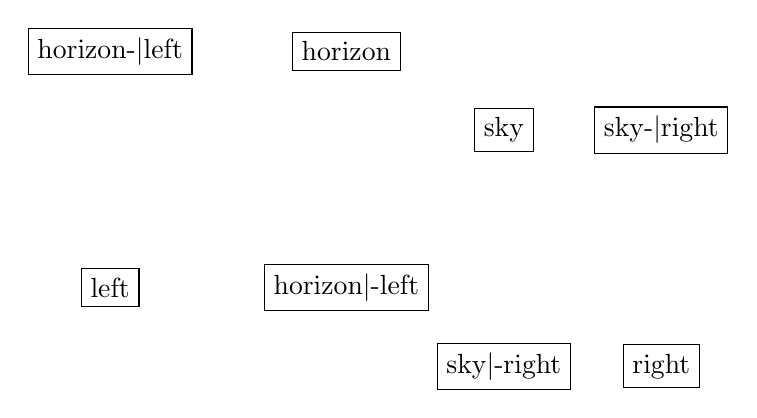
\begin{tikzpicture}
\coordinate (horizon) at (3,0);
\coordinate (sky) at (5,-1);
\coordinate (left) at (0,-3);
\coordinate (right) at (7,-4);

\node [draw](horizon) at (3,0) {horizon};
\node [draw](sky) at (5,-1) {sky};
\node [draw](left) at (0,-3) {left};
\node [draw](right) at (7,-4) {right};

\node [draw] at(horizon -| left) {horizon-\textbar left};%0,0
\node [draw] at(horizon |- left) {horizon\textbar-left};%3,-4
\node [draw] at(sky -| right) {sky-\textbar right};%6,-1
\node [draw] at(sky |- right) {sky\textbar-right};%3,-4
\end{tikzpicture}
\caption{-\textbar~和\textbar-运算符含义的确定}
\end{figure}

经过我的分析\footnote{没错,是一点点儿试出来的经验公式},-\textbar 和\textbar -
运算符号遵循下列规律:

\begin{equation}
(x_1,y_1) \dashv (x_2,y_2) = (x_2,y_1)
\end{equation}
%(x_1,y_1) -| (x_2,y_2) = (x_2,y_1)

\begin{equation}
(x_1,y_1) \vdash (x_2,y_2) = (x_1,y_2)
\end{equation}

所以你应该知道(sky -\textbar ~right)得到的结果就是与right相同的横坐标,与sky相同
的纵坐标的那个点。

那么,另外一个点呢?([yshift=-5mm]horizon-\textbar ~left)得到的应该是left的横坐
标和horizon的纵坐标决定的那个点么?显然不是,要不[yshift=-5mm]有什么用。从字面意
思上很容易猜测到这个是什么,yshift=-5mm应该表示纵坐标移动-5mm,也就是向y轴负轴移
动5mm的距离。
yshift以及xshift属于Transformations概念,其定义如下:
\begin{equation}
(x,y) \stackrel{xshift}{\longrightarrow}(\textbf{factor}+x,y)
\end{equation}
\begin{equation}
(x,y) \stackrel{yshift}{\longrightarrow}(x,\mathbf{factor}+y)
\end{equation}
\begin{equation}
(x,y) \stackrel{shift}{\longrightarrow}(\textbf{factor}+x,\mathbf{factor}+y)
\end{equation}



这样解释完美么?并不是。此时还涉及到一个优先级的问题:[yshift=-5mm]先和horizon坐
标结合,之后参与与left的-\textbar 运算呢,还是horizon先和left做-\textbar 运算,
得到的结果在[yshift=-5mm]?显然这两种解释的结果都一样,因为无论先后,最后得到的
结果其纵坐标始终是horizon的纵坐标减去5mm。不过如果不搞清楚这个问题我们是无法进行
认真细致的学习的。你可以尝试将yshift改成xshift,如果点位置不变,那么就是第一种解
释,即[]的优先级大于-\textbar 的优先级;如果点位置变了,那么就是第二种解释,即
-\textbar 优先级大于[]的优先级。我得到的结果是位置改变,也就是说\uwave{-\textbar
(和\textbar -)的优先级大于[]运算优先级}。记住这个结论,因为它很重要。

\begin{figure}[htbp]
\centering
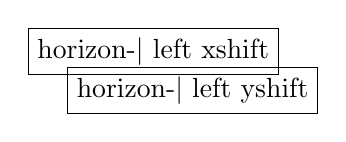
\begin{tikzpicture}
\coordinate (horizon) at (3,0);
\coordinate (left) at (0,-4);
\node [draw] at([yshift=-5mm]horizon -| left) {horizon-\textbar~left yshift};%0,0
\node [draw] at([xshift=-5mm]horizon -| left) {horizon-\textbar~left xshift};%0,
\end{tikzpicture}
\caption{运算符优先级确定}
\end{figure}

之后第20行到第23行同样是关于渐变色绘制的,只不过这个矩形是由四个点组成,(front
-\textbar ~left),(horizon -\textbar~left),(horizon -\textbar~right),(front
-\textbar~right)。
不过(horizon -\textbar~left)与(horizon -\textbar~right)之间的直线路径使用了装饰
(decorate),住所内更是样式为random steps。效果如下:

\begin{figure}[htbp]
\centering
\tikz \draw [decorate,decoration=random steps,color=blue] (0,0) -- (5,0);
\caption{random steps的装饰效果示意}
\end{figure}

第24,25两行同样使用矩形渐变色,矩形坐标的确立与之前所讲述的别无二致,而第26
行颜色填充矩形,同样的道理,在此不再多说。

\section{倒影文字效果}

第28行到第34行,自定义了nodeshadowed命令,最终展示的效果就是封面上标题以及其倒影
的效果。以下为其代码:

\lstinputlisting[firstline=28,lastline=34,firstnumber=28]{pgfmanualtitlepage.tex}

这里先预定义了一个nodeshadowed,然后四次引用。因而只要弄清楚nodeshadowed是如何作
用的,这一部分就可以说彻底清楚明白了。

我们先解释一下第30行和第32行出现的yslant操作。yslant操作和之前的yshift操作一样,
属于坐标变换范畴,在manual中,分类都为第217页,21章Transformations。yslant核心在
于slant,倾斜,除了yslant,显然与之对偶还有xslant。xslant和yslant坐标变换定义如
下:
\begin{equation}
(x,y) \stackrel{xslant}{\longrightarrow}((1+\mathbf{factor})*x,y)
\end{equation}
\begin{equation}
(x,y) \stackrel{yslant}{\longrightarrow}(x,(1+\mathbf{factor})*y)
\end{equation}

$(0,0)$无论如何变化,其结果还是$(0,0)$。

为方便起见,我们假定有一个\verb|\nodeshadowed [at={(0,1)}]{A};|这个命令,代入
nodeshadowed的定义中,展开可获得如下结果:
\begin{Verbatim}
{
\node[scale=2,above,at={(0,1)}]{A};
\node[scale=2,above,at={(0,1)},yscale=-1,scope fading=south,opacity=0.5]{A};
}
\end{Verbatim}

\begin{figure}[htbp]
\centering
\begin{tikzpicture}
{
\node[scale=2,above,at={(0,1)}]{倒影效果};
\node[scale=2,above,at={(0,1)},yscale=-1,scope fading=south,
fading angle=45,opacity=0.5]{倒影效果};
}
\end{tikzpicture}
\caption{倒影效果示例}
\end{figure}

这里还有一个scale(缩放)操作,也属于Transformations之列,其定义如下:
\begin{equation}
(x,y) \stackrel{scale}{\longrightarrow}(\textbf{factor}*x,\mathbf{factor}*y)
\end{equation}
此外还有单独的xscale和yscale操作,定义如下:
\begin{equation}
(x,y) \stackrel{xscale}{\longrightarrow}(\textbf{factor}*x,y)
\end{equation}
\begin{equation}
(x,y) \stackrel{yscale}{\longrightarrow}(x,\mathbf{factor}*y)
\end{equation}

above操作位于pgfmanual第155页,等同于$anchor=south$,可以用$above=offset$的方式
指定与之距离。如果不指定above的值,默认为0pt。above相对的位置由之后的at或者其他
节点的位置确定,在本例子中则为at所确定的绝对坐标。

上述展开的两个节点,第一个节点是在(0,1)坐标纸上写一个A,然后将此放大两倍。而第二
个节点除此之外,$yscale=-1$将节点翻转。其余需要解释的,也不过是scope fading和
opacity了。

opacity(不透明度)同时设置draw opacity(绘制线的不透明度)和fill opacity(填充颜色的
不透明度)两个的值。scope fading则指明向south方向不透明度渐变。事实上这两个选项的
结合就形成了封面所示的那种倒影的效果。

对于Tikz和PGF这两组文字使用了yslant=0.05和yslant=-0.05效果,使之Tikz右边轻微向上
,而PGF左边轻微向上,达到了拱卫中间\&字符的目的。如果不明显,你可以试着把yslant
的值更改得大一些,然后就很清楚了。

非常遗憾的是,scope fading=south在我这里似乎无法工作,无论加上与否出来的倒影都没
有渐变效果。如果你知道为什么,请联系我,我的邮箱是lanphon@gmail.com,非常感谢。

\section{雪花效果}

封面最上有蓝天飘着雪花的效果,仔细观察那些雪花,十分漂亮,戴着梦幻般的色彩。而这
一切都是由如下的几句话实现的:

\lstinputlisting[firstline=35,lastline=47,firstnumber=35]{pgfmanualtitlepage.tex}

第36行指定填充操作,颜色为白色,修饰形状为Koch snowflake,不透明度0.9。Koch
snowflake修饰操作可参见manual第270页的讲解。而40到46行则使用了三次嵌套的修饰操
作,得到一个雪花的图案。第43行指定坐标从(0,0)开始,顺时针旋转60度,取长度为1,逆
时针旋转60度,同样去长度为1,然后连成封闭图形,这样我们就可以得到一个正三角形。
接着三次decorate操作,在正三角形的基础上生长出雪花,过程如下所示\footnote{原来雪
花颜色为白色而背景色为蓝色,现在背景为白色,为方便观察,将雪花填充颜色改为蓝色}:

\begin{figure}[htbp]
\centering
\subfloat[无修饰]{
\begin{tikzpicture}
\fill [blue,decoration=Koch snowflake,opacity=.9]
{
(0,0) -- ++(60:1) -- ++(-60:1) -- cycle
};
\end{tikzpicture}
}
\hspace{15pt}%
\subfloat[一次修饰]{
\begin{tikzpicture}
\fill [blue,decoration=Koch snowflake,opacity=.9]
decorate {
(0,0) -- ++(60:1) -- ++(-60:1) -- cycle
};
\end{tikzpicture}
}
\hspace{15pt}%
\subfloat[二次修饰]{
\begin{tikzpicture}
\fill [blue,decoration=Koch snowflake,opacity=.9]
decorate {
decorate {
(0,0) -- ++(60:1) -- ++(-60:1) -- cycle
}
};
\end{tikzpicture}
}
\hspace{15pt}%
\subfloat[三次修饰]{
\begin{tikzpicture}
\fill [blue,decoration=Koch snowflake,opacity=.9]
decorate {
decorate {
decorate {
(0,0) -- ++(60:1) -- ++(-60:1) -- cycle
}
}
};
\end{tikzpicture}
}
\caption{雪花形状生成示意图}
\end{figure}

第35行指定一个foreach循环,i的值从0.5以步长0.1增长到2,关键就在于第37行到39行的
内容了。36行,shift=(horizon)先将绘图原点搬到了horizon处,事实上所有的雪花都是在
horizon之上才出现。然后shift=\{(rand*11,rnd*7)\}操作。rand产生一个落到(-1,1)之间
的伪随机序列,而rnd则产生一个落到(0,1)之间的伪随机序列,两个函数的说明参见
manual的414页。当然,随机数还需要乘上一个放大因子。我们看到横坐标使用rand伪随机
序列,以使雪花铺满从左到右的空间。而纵坐标使用rnd伪随机序列,确保雪花只出现在
horizon之上。scale=\textbackslash i则将雪花缩放,最小的为原来的一半,最大的为原
来的两倍,并且没有一个雪花是相同大小的。

第38行开始,double copy shadow操作位于manual第309页。copy shadow意为复制性投影,
而double copy shadow则有双重投影。投影不透明度(opacity)为0.2,并且投影的x坐标保
持不变,y坐标去偏离3*\textbackslash i pt,填充白色,draw=none则表示无绘制曲线。

\begin{figure}[htbp]
\centering
\begin{tikzpicture}
\fill [blue,decoration=Koch snowflake,opacity=.9]
[scale=5]
[double copy shadow={opacity=0.5,shadow xshift=6pt,
shadow yshift=8pt,fill=red,draw=green}]
decorate {
decorate {
decorate {
(0,0) -- ++(60:1) -- ++(-60:1) -- cycle
}
}
};
\end{tikzpicture}
\caption{双重复制性投影效果}
\label{fig:doublecopy}
\end{figure}

第\pageref{fig:doublecopy}页图\ref{fig:doublecopy}给出了双重投影效果的示意图,为
观察到绘制边线,雪花在原来的基础上放大了5倍。雪花本身为蓝色,但投影为红色,而边
线绘制则为绿色,投影的不透明度为0.5,横坐标移动6pt,纵坐标移动8pt。之所以展示一个
并不好的配色方案绘制而成的雪花只是想弄明白各个参数具体的含义。从图中我们可以看出
opactiy这个参数是在前一个的基础上继续不透明,所以两个投影的不透明度并不一致。

\section{万径人踪灭:脚印绘制}

源码从48行起,至146行,均为封面下放文字的添加,使用了listings环境,在此不再赘述
。最后要将的就是下放雪地里的两行足迹的绘制。

\lstinputlisting[firstline=147,lastline=155,firstnumber=147]{pgfmanualtitlepage.tex}

既然是两行足迹,那么刚好和两个fill一致,我们只需要弄明白一个的道理,另外一个
就是同理可得了。

147行开始,指明填充,有修饰操作,修饰为脚印(footprints),之后指明脚印类型为gnome
,足迹不透明度为0.5,棕色(brown)。路径则为(left text.south)到(right text.north)
,出发切线角度为-45度,到达切线角度为135度。关于out和in的具体含义参见manual第367
页。left text和right text就是前文提到的省略去掉的左右两边的文字说明。而out和in所
制定的曲线角度则是相对于(left text.south)与(right text.north)的连线而言的。

\begin{figure}[htbp]
\centering
\begin{tikzpicture}[scale=.6]
\coordinate (left text) at (0,-2);
\coordinate (right text) at (4,0);

\draw (left text) to [out=-45,in=110] (right text);
\end{tikzpicture}
\caption{out,in参数确定曲线的形状}
\label{fig:outin}
\end{figure}

\autoref{fig:outin}给出了out参数和in参数来绘制光滑曲线的一个例子。本例子中
begin坐标为(0,-2),end坐标为(4,0),out=-45,in=110。我们可以在路径绘制的过程中使
用decorate操作,用脚印来填充。如\autoref{fig:footprint}所示。

\begin{figure}[htbp]
\centering
\begin{tikzpicture}[scale=.6]
\coordinate (left text) at (0,-2);
\coordinate (right text) at (4,0);

\fill [decorate,decoration=footprints,
decoration={footprints,foot length=6pt,foot of=gnome},
opacity=.9,brown]
(left text) to [out=-45,in=110] (right text);
\end{tikzpicture}
\caption{使用脚印修饰路径}
\label{fig:footprint}
\end{figure}

第151行开始则是另外一组的足迹了,与之前的一组足迹相比,多了一些例如foot angle,
foot length等的参数,这些都是一些细节性的问题。关于足迹绘制的所有参数请参见
manual第271页足迹修饰一章。

\section{写在最后}

经过几天辛苦的努力,终于把这篇文档整理完毕了。学习tikz,从某种意义上来讲开始的时
候依然是学习一门新的编程语言。我认为所有的语言,仅凭看书是什么都学不会的。最好的
学习方法莫过于从示例中学习,遇到不懂的去查询手册,做好整理工作。多学习几个例子,
这门编程语言也就学完了。

但tikz的学习也不止于此,若tikz基本使用方法学习完毕,想要绘制出如同pgfmanual封面
一样精美的图形对我等而言仍然是个不小的工作。此时,程序性质的东西已经不再重要,这
里已经是艺术性的层次了:页面布局,元素选择,配色方案,效果设计,等等等等。艺术般
的设计需要艺术般的才华,而这种艺术性的思想却不是学习编程一样,一朝一夕可以获得的
。它必须经过长时间的积累,尝试与总结,方可小有所成。同时,借鉴别人的设计思想,也
是提升自己品味的一个重要手段:认真观察他人是如何选择不同的布局与配色的,某些元素
放到这里究竟表达了怎样的一种含义,诸如此类,不一而足。

学无止境,艺术性的追求足以让我们穷尽一生,而更高处,还会有怎样的风景等待着我们呢
?每个人应该都会有自己的想法吧。

\section{致谢}

首先感谢CTeX论坛各位版众热心的帮助。我也是看着论坛上的帖子,一步一步逐渐走到现在
的。

感谢xuanyuan\_ying,指正1.0版本中的一个错误以及帮助测试渐变色。

\clearpage
\phantomsection
\addcontentsline{toc}{section}{附:封面设计实现以及源码}
\section*{附:封面设计实现以及源码}

\lstinputlisting{pgfmanualtitlepage.tex}
\clearpage
{
\parindent0pt
\null
\colorlet{mintgreen}{green!50!black!50}

\thispagestyle{empty}
\vskip3cm
\vfill
\hfil
\begin{tikzpicture}[overlay]
\coordinate (front) at (0,0);
\coordinate (horizon) at (0,.31\paperheight);
\coordinate (bottom) at (0,-.6\paperheight);
\coordinate (sky) at (0,.57\paperheight);
\coordinate (left) at (-.51\paperwidth,0);
\coordinate (right) at (.51\paperwidth,0);

\shade [bottom color=blue!30!black!10,top color=blue!30!black!50]
([yshift=-5mm]horizon -|  left) rectangle (sky -| right);
\shade [bottom color=black!70!green!25,top color=black!70!green!10]
(front -| left) -- (horizon -| left)
decorate [decoration=random steps] { -- (horizon -| right) }
-- (front -| right) -- cycle;
\shade [top color=black!70!green!25,bottom color=black!25]
([yshift=-5mm-1pt]front -| left) rectangle ([yshift=1pt]front -| right);
\fill [black!25] (bottom -| left) rectangle ([yshift=-5mm]front -| right);

\def\nodeshadowed[#1]#2;{\node[scale=2,above,#1]{#2};\node[scale=2,above,#1,yscale=-1,scope fading=south,opacity=0.4]{#2};}

\nodeshadowed [at={(-5,5  )},yslant=0.05] {\Huge Ti\textcolor{orange}{\emph{k}}Z};
\nodeshadowed [at={( 0,5.3)}] {\huge \textcolor{mintgreen}{\&}};
\nodeshadowed [at={( 5,5  )},yslant=-0.05] {\Huge \textsc{PGF}};
\nodeshadowed [at={( 0,2  )}] {Manual for Version \pgftypesetversion};

\foreach \i in {0.5,0.6,...,2}
\fill [white,decoration=Koch snowflake,opacity=.9]
[shift=(horizon),shift={(rand*11,rnd*7)},scale=\i]
[double copy shadow={opacity=0.2,shadow xshift=0pt,shadow
yshift=3*\i pt,fill=white,draw=none}]
decorate { 
decorate { 
decorate {
(0,0) -- ++(60:1) -- ++(-60:1) -- cycle
}
}
};

\node (left text) [text width=.5\paperwidth-2cm,below right,at={(-.5\paperwidth+1cm,-1.5cm)}]
{
\fontfamily{pcr}
\def\textbraceleft{\char`\{}
\def\textbraceright{\char`\}}
\def\textbackslash{\char`\\}
\begin{lstlisting}[basicstyle=\scriptsize\color{black},
keywordstyle=\bfseries\color{white},
identifierstyle=\bfseries\color{black},
keywords={tikzpicture,shade,fill,draw,path,node},
literate={-}{{-}}1]
\begin{tikzpicture}
\coordinate (front) at (0,0);
\coordinate (horizon) at (0,.31\paperheight);
\coordinate (bottom) at (0,-.6\paperheight);
\coordinate (sky) at (0,.57\paperheight);
\coordinate (left) at (-.51\paperwidth,0);
\coordinate (right) at (.51\paperwidth,0);

\shade [bottom color=white,
top color=blue!30!black!50]
([yshift=-5mm]horizon -|  left)
rectangle (sky -| right);

\shade [bottom color=black!70!green!25,
top color=black!70!green!10]
(front -| left) -- (horizon -| left)
decorate [decoration=random steps] {
-- (horizon -| right)  }
-- (front -| right) -- cycle;

\shade [top color=black!70!green!25,
bottom color=black!25]
([yshift=-5mm-1pt]front -| left)
rectangle ([yshift=1pt]front -| right);

\fill [black!25]
(bottom -| left)
rectangle ([yshift=-5mm]front -| right);

\def\nodeshadowed[#1]#2;{
\node[scale=2,above,#1]{#2};
\node[scale=2,above,#1,yscale=-1,
scope fading=south,opacity=0.4]{#2};
}
\end{lstlisting}
};

\node (right text) [text width=.5\paperwidth-2cm,below right,at={(1cm,-1.5cm)}]
{
\fontfamily{pcr}
\def\textbraceleft{\char`\{}
\def\textbraceright{\char`\}}
\def\textbackslash{\char`\\}
\begin{lstlisting}[basicstyle=\scriptsize\color{black},
keywordstyle=\bfseries\color{white},
identifierstyle=\bfseries\color{black},
keywords={tikzpicture,shade,fill,draw,path,node},
literate={-}{{-}}1]
\nodeshadowed [at={(-5,8  )},yslant=0.05]
{\Huge Ti\textcolor{orange}{\emph{k}}Z};
\nodeshadowed [at={( 0,8.3)}]
{\huge \textcolor{green!50!black!50}{\&}};
\nodeshadowed [at={( 5,8  )},yslant=-0.05]
{\Huge \textsc{PGF}};
\nodeshadowed [at={( 0,5  )}]
{Manual for Version \pgftypesetversion};

\foreach \i in {0.5,0.6,...,2}
\fill
[white,opacity=\i/2,
decoration=Koch snowflake,
shift=(horizon),shift={(rand*11,rnd*7)},
scale=\i,double copy shadow={
opacity=0.2,shadow xshift=0pt,
shadow yshift=3*\i pt,
fill=white,draw=none}]
decorate {
decorate { 
decorate { 
(0,0)- ++(60:1) -- ++(-60:1) -- cycle
} } };

\node (left text) ...
\node (right text) ...

\fill [decorate,
decoration={footprints,foot of=gnome},
opacity=.5,brown] (left text.south)
to [out=-45,in=135]    (right text.north);
\fill [decorate,
decoration={footprints,foot of=felis silvestris,
foot length=5pt,stride length=15pt,foot angle=0},
opacity=.5,green!50!black] (left text.south)
to [out=20,in=180] (right text.north west);
\end{tikzpicture}
\end{lstlisting}
};

\fill [decorate,decoration=footprints,
decoration={footprints,foot of=gnome},
opacity=.5,brown] (left text.south)
to [out=-45,in=135]    (right text.north);
\fill [decorate,decoration={footprints,foot length=5pt,foot of=felis
silvestris,stride  length=15pt,foot angle=0},
opacity=.5,green!50!black] (left text.south)
to [out=20,in=180] (right text.north west);
\end{tikzpicture}
\vfill
\vbox{}
\clearpage
}


\end{document}
